% !TEX encoding = UTF-8 Unicode
%\chapter{Implementação}
\xchapter{IImplementação}{}
\acresetall
	
	Neste capítulo serão descritos alguns detalhes de implementação, além de descrever os testes realizados. A seção sobre os detalhes de implementação visa esclarecer como alguns problemas foram atacados, complementando as soluções abordadas no capítulo \ref{cap:especificacao}. A seção sobre testes abordará sobre em quais condições estes foram executados, os objetivos e os procedimentos adotados.

\section{Detalhes da implementação}

	A seguir serão descritos alguns problemas e suas respectivas soluções que não foram abordados nas seções anteriores. Estes problemas não foram abordados anteriormente visto que suas soluções estão no nível da implementação.
	
\subsection{Colhendo informações de QoS}
	
	Como já foi dito anteriormente, o protocolo utilizado para colher informações relativas a QoS nos roteadores foi o SNMP. Este último foi utilizado para colher informações relativas ao \textit{Diffserv} configurado no roteador. Tais informações são estatísticas colhidas pelo agente do SNMP e armazenadas nas MIBs. Apesar de existirem MIBs proprietárias para colher informações relativas ao \textit{Diffserv}, a IETF padronizou uma MIB para a arquitetura do \textit{Diffserv} \cite{BCS02}.
	
	Como em nosso ambiente de teste foi utilizado um roteador da Cisco modelo 871, a MIB utilizada para captura de informações relativas a QoS foi a MIB proprietária \textit{CISCO-CLASS-BASED-QOS-MIB} \cite{MIBCISCO08} definida pela própria Cisco.
	
\subsubsection{CISCO-CLASS-BASED-QOS-MIB}
		
		Esta MIB provê acesso de leitura para informações de configuração e de estatísticas referente às classes de tráfego configuradas no roteador. As informações de configuração dessa MIB incluem todos os parâmetros relativos às classes, políticas e critérios de seleção configurados no roteador (para entender melhor estes conceitos e suas relações assim como a forma como estes são utilizados, veja o Apêndice \ref{apend:relacionamentos_MIB}). As estatísticas disponíveis nesta MIB incluem contadores (tais como quantidades de pacotes descartados) relativos às classes de tráfego antes e depois das políticas de QoS serem aplicadas. Uma das variáveis definidas nesta MIB é a seguinte:
		
\begin{itemize}
\item \textbf{cbQosCMDropPkt}: Este objeto MIB (cujo OID é 1.3.6.1.4.1.9.9.166.1.15.1.1.13) armazena o número de pacotes descartados por classe decorrentes a todas as características que causam descartes (como policiamento). Essas caracterísiticas são aquelas responsáveis por prover a funcionalidade necessária para implementar o \textit{Diffserv}.
\end{itemize}

\subsubsection{Descobrindo se a QoS está sendo degradada}
	
	A degradação da QoS dos canais \textit{TIMELY} é decorrente do mal fornecimento do serviço Expresso. Esse mal fornecimento pode ocorrer quando a classe que recebe o serviço Expresso está sobrecarregada. A sobrecarga faz com que componenetes do \textit{Diffserv} como o policiamento e reguladores de fluxo (\textit{Traffic Shaping}) causem descartes, compromentendo o serviço. Mesmo sabendo que o serviço Expresso conta com largura de banda garantida e que os roteadores de borda são responsáveis por garantir que as SLAs sejam respeitadas, em nosso ambiente de teste existe apenas um roteador, sendo assim nós não contamos com os roteadores de borda, havendo a possibilidade do serviço ser comprometido devido à sobrecarga.
	
	Nós verificamos se houve degradação da seguinte maneira: o QoSPA envia duas mensagens SNMP, cada uma requisitando o valor do objeto MIB \textit{cbQosCMDropPkt}. Calculamos a diferença entre os dois valores. Se a diferença for maior do que zero, pacotes estão sendo descartados e o serviço está comprometido (a QoS não está sendo mantida), caso contrário, a QoS dos canais que recebem tal serviço está sendo mantida. Como já foi comentado anteriormente, o QoSPA monitora periodicamente o roteador ao qual está vinculado (na verdade, assim que um monitoramento é finalizado, logo em seguida outro é executado). Sendo assim, cada vez que o monitoramento é executado, o QoSPA não necessita enviar duas mensagens SNMP requisitando o valor do objeto MIB \textit{cbQosCMDropPkt}. Ele envia apenas uma mensagem e a diferença é calculada a partir do valor obtivo no monitoramento anteriormente executado. É importante observar que caso ambiente Diffserv esteja completo (composto por roteadores de borda e roteadores de núcleo), este tipo de degradação mencionado anteriormente não aconteceria, mas o SNMP poderia ser utilizado para colher valores de outros objetos MIB que também forneçam uma informação mais robusta acerca da degradação, como por exemplo verificar o corrompimento do \textit{buffer}.
	
	Para que as mensagens SNMP do tipo \textit{SNMPGET} possam ser enviadas requisitando a quantidade de pacotes descartados da classe que recebe o serviço Expresso, antes é necessário que índices relativos à esta classe sejam capturados. Para saber como ocorre este procedimento, veja o Apêndice \ref{apend:indices_MIB}.

\subsection{Otimizando o monitoramento do QoSPA}	

	Vários canais de comunicação \textit{TIMELY} passam pelo mesmo roteador. Sendo assim, durante o processo de monitoração (executado através das funções \textit{QOS} e \textit{VerifyChannel}), vários QoSP podem requisitar dentro de um intervalo de tempo curto informações de QoS ao mesmo QoSPA. Além do mais, no processo de monitoração da QoS de um canal, o monitoramento executado pelo QoSPA junto ao roteador possivelmente será um gargalo, visto que as mensagens do protocolo SNMP são maiores comparadas às mensagens do protocolo definido para o QoSPM, além do processamento executado pelo roteador ser mais lento se comparado aos \textit{hosts}.
	
	Para tentar otimizar o monitoramento realizado pelo QoSPA, duas medidas foram tomadas: o monitoramento é contínuo, sendo assim, quando uma solicitação por parte de um QoSP chega requisitando saber se a QoS continua sendo mantida, esta requisição se utilizará do monitoramento em execução, caso a resposta do roteador ainda não tenha chegado. Além do monitoramento ser contínuo, todas as requisições que chegam enquanto o monitoramento está sendo executado e, principalmente, se a resposta do roteador ainda não chegou, são armazenadas em um \textit{buffer}. Ao fim do monitoramento, as requisições se utilizarão da resposta deste monitoramento.

%falando sobre o TrafficListener	
\subsection{Escutando os canais de comunicação}	

	Para que a função $VerifyChannel(c_{x/y})$ (descrita no capítulo \ref{cap:qos_provider}) possa ser implementada corretamente, é necessário que seja verificada a existência de tráfego no canal. Como foi descrito na seção que aborda a modelagem do QoSPM, a entidade \textit{Traffic Listener} é responsável por esta função. Para que fosse possível armazenar as informações relativas à ocorrência de tráfego, duas funções foram definidas a serem utilizadas pelos processos aplicativos (que executam sobre o modelo HA) na hora de enviar e receber mensagens pelos seus canais de comunicação, criados junto ao QoS \textit{Provider}. Tais funções são:
	
\begin{itemize}
\item $qosp\_sendmsg$: utilizada para enviar uma mensagem pelo canal de comunicação. Ela é apenas um invólucro para as funções $sendmsg$ e $rt\_dev\_sendmsg$. $sendmsg$ faz parte da API do linux para programação em redes, sendo utilizada para envio de mensagens em um \textit{socket}. $rt\_dev\_sendmsg$ faz parte da API do RTnet, sendo utilizada para envio de mensagens em um \textit{socket} de tempo real. Antes de executar uma das funções que estão sendo involucradas, $qosp\_sendmsg$ atualiza a informação da hora da última mensagem trocada no canal com a hora local.

\item $qosp\_recvmsg$: utilizada para receber uma mensagem pelo canal de comunicação. Ela é apenas um invólucro para as funções $recvmsg$ e $rt\_dev\_recvmsg$. $recvmsg$ também faz parte da API do linux para programação em redes, sendo utilizada para o recebimento de mensagens em um \textit{socket}. $rt\_dev\_recvmsg$ faz parte da API do RTnet, sendo utilizada para o recebimento de mensagens em um \textit{socket} de tempo real. Depois de executar uma das funções que estão sendo involucradas, $qosp\_recvmsg$ atualiza a informação da hora da última mensagem trocada no canal com a hora local.
\end{itemize}

	Cada função é um invólucro para duas funções, visto que dependendo da QoS do canal de comunicação utilizado pelo processo para enviar ou receber mensagem, a comunicação se dará no contexto de tempo real (API do RTNet) quando o canal for \textit{TIMELY} ou no contexto do Linux quando for \textit{UNTIMELY}. Ambas as funções definidas acima possuem tanto os mesmos parâmetros como o mesmo tipo de retorno das funções das quais elas são invólucros, exceto por um parâmetro adicional que corresponde a um descritor de canal. Para cada canal do processo aplicativo que teve sua QoS alterada para \textit{TIMELY}, ele obtém um descritor para este canal que será utilizado como parâmetro nas funções de envio e recepção de mensagens por este canal, sendo que este parâmetro só será utilizado quando o canal for \textit{TIMELY}.
	
\section{Testes}	

\begin{figure}
\centering
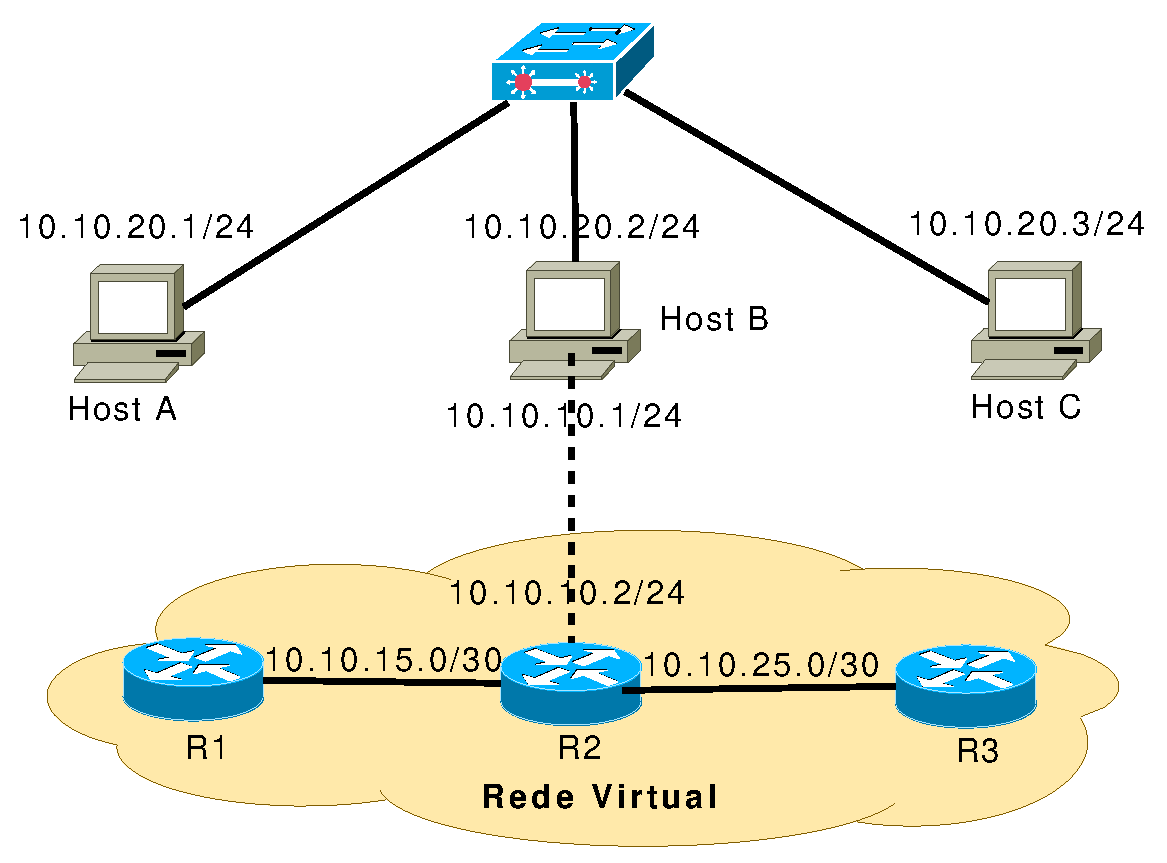
\includegraphics[scale=0.7]{ambiente_teste}
\caption{Ambiente de teste}
\label{fig:ambiente_teste}
\end{figure}

	Devido às dificuldades encontradas (ver capítulo \ref{cap:conclusao}), medições não puderam ser realizadas para que resultados fossem colhidos. Alguns testes foram realizados na medida do possível. Testes de integração foram realizados para verificar se os componentes do QoSPM estavam se comunicando corretamente.
	
	Para testar o QoSPM, nós utilizamos o laboratório localizado no módulo 2 do Lasid, pertencente ao projeto \textit{Um Modelo Híbrido e Adaptativo Tolerante à Falhas}. O laboratório é composto por três computadores e um \textit{switch} (Figura \ref{fig:ambiente_teste}), sendo que uma rede local (10.10.20.0) foi configurada com os três computadores.
	
	Existem três componentes QoSP executando na rede, um para cada \textit{host}. Além disso, existe um componente QoSPA executando no \textit{Host} B. O \textit{Host} B servirá tanto como hospedeiro para um QoSP como para um QoSPA, visto que não haviam máquinas suficientes. Além de hospedar os componentes citados anteriormente, o \textit{Host} B também passa a ser visto pelos componentes QoSP (inclusive pelo QoSP que executa em seu \textit{host}) como o roteador da rede. É importante salientar que o \textit{Host} B não se comporta como um roteador (visto que o mesmo não rotea pacotes e apenas uma rede local foi configurada). O \textit{Host} B é visto como roteador pelos QoSP para que os detectores de defeitos que executam nos mesmos possam ter um elemento a mais para monitorar.
	
	O roteador que havia sido adquirido para o projeto (um modelo 871 da Cisco) acabou não pudendo ser utilizado (para maiores detalhes ver capítulo \ref{cap:conclusao}). Para testar o monitoramento dos roteadores através do SNMP foi utilizado o Dynamips/Dynagen \cite{DYNAGEN08}. O Dynamips permite emular uma rede composta por roteadores Cisco, além de outros elementos de rede como \textit{switches}, em um computador. O Dynagen corresponde a um \textit{front-end} para o Dynamips, permitindo a configução de um laboratório de rede facilmente. Com a utilização do Dynamips foi possível criar uma rede virtual (Figura \ref{fig:ambiente_teste}) composta por três roteadores. O roteador R2 representa o roteador vinculado ao QoSPA, enquanto que R1 e R3 foram criados apenas para sobrecarregar R2. A rede virtual está "ligada" ao \textit{Host} B através de R2 (observe que a rede virtual está hospedada no \textit{Host} B e é vista apenas por ele), sendo que R2 era acessado através de uma interface virtual (10.10.10.1/30) criada com o \textit{tunctl}. O \textit{tunctl} é um comando utilizado para criar dispositivos TUN/TAP, sendo que estes dispositivos correspondem a \textit{drivers} que implementam dispositivos de rede através de \textit{software}, não necessitando de um adaptador de rede. TAP simula um dispositivo \textit{Ethernet} e opera na camada 2, enquanto o TUN simula um dispositivo da camada de rede e opera na camada 3. É importante salientar que o roteador virtual criado é visto apenas pelo QoSPA e serve apenas para testar o monitoramento executado pelo mesmo. Este roteador criado fornece funcionalidades semelhantes ao modelo 871 da Cisco, inclusive dando suporte à CISCO-CLASS-BASED-QOS-MIB.

	Para testar as funções \textit{QoS} e \textit{VerifyChannel} (ver capítulo \ref{cap:qos_provider}), um canal de comunicação foi definido, sendo este formado pelo processo $p_{x}$ que executa no \textit{Host} A, e $p_{y}$ que executa no \textit{Host} B. Os processos ficam trocando mensagens entre si periodicamente. A função \textit{VerifyChannel} foi executada no \textit{Host} C para verificar o estado do canal $c_{x/y}$, sendo assim, tanto a função \textit{VerifyChannel} como a própria função \textit{QoS} foram testadas. Os valores retornados pela função \textit{Delay} assim como o o intervalo de tempo durante o qual um canal deve ser investigado para verificar se houve tráfego foram configurados aleatoriamente, visto que o intuito era testar a integração entre os componentes.
	
	Para testar se a degradação era detectada, os roteadores R1 e R3 foram criados para sobrecarregar o roteador R2. R1 ficava enviando periodicamente mensagens \textit{ECHO REQUEST} para R3 enquanto que  R3 ficava enviando periodicamente mensagens do mesmo tipo no sentido inverso. Os pacotes ICMP (\textit{ECHO REQUEST}) foram configurados para receber o Serviço Expresso, sendo que este estava vinculado às interfaces 10.10.15.1 e 10.10.25.1 (na direção da saída) de R2. Quando o QoSPA requisitava informações da quantidade de pacotes descartados, sendo que esta requisição era feita no contexto da execução da função \textit{QoS}, o QoSPA percebia a degradação e notificava a degradação.